\chapter{Thermodynamik (Wärmelehre)}
Gesetz der Mechanik angewandt auf sehr viele Teilchen

\section{Modell des idealen Gases}
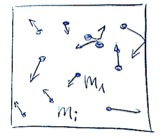
\includegraphics{Bild108} \\
$N$ teilchen \\
ideales Gas
\begin{itemize}
	\item Teilchen punktförmig
	\item WW nur während Stössen
\end{itemize}
$m_i , \vec{r_i}(t) , \vec{v_i}(t) \implies$ vollständige Beschreibung \\
$\implies$ ist irrelevant (unmöglich bei $N \approx 10^{23}$ ) \\
TD: Wichtige Grössen des gesamten Gases, die sich zeitlich nicht ändern!

\subsection{Zustandsgrössen}
\begin{description}
	\item[Innere Energie]
		\[ U = \sum_{i = 1}^N \frac{1}{2} m_i v_i^2 \overset{!}{=} \text{ konst.} \]
		Wieso? \\
		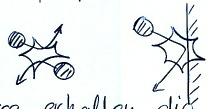
\includegraphics{Bild109} \\
		Einzelstösse erhalten kinetische Energie!
	\item[mittlere Energie pro Teilchen]
		\[ \overline{E_{\text{kin}}} = \frac{1}{2} \overline{mv^2} = \frac{U}{N} \]
\end{description}

\subsection{Die Geschwindigkeitsverteilung}
Nicht alle Teilchen sind gleich schnell! \\
Zufallsbewegung, Stösse \\
$\implies$ Verteilung im Gas \\
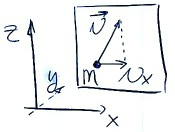
\includegraphics{Bild110} \\
Histogramm! \\
$v_x$ ist Zufallsvariable \\
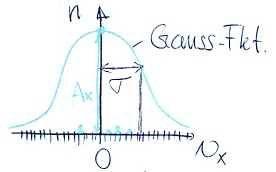
\includegraphics{Bild111} \\
Normalverteilung
\[ 
	n(v_x) = A_x e^{-\frac{v_x^2}{2\sigma^2}} \\
	v_x = \sigma \\
	n(\sigma) = A_x e^{-\frac{1}{2}} \approx 0.6 \cdot A_x
\]
$\implies$ $v_x$-Verteilung bleibt konstant, die einzelnen Teilchen änder dauernd $\vec{v}$. \\
$\implies$ Mittelwert $\overline{v_x} = 0$ \\
Wichtiger: Verteilung der Schnelligkeit
\[
	v = \sqrt{v_x^2 + v_y^2 + v_z^2} \geq 0
	\intertext{Resultat:}
	n(v) = A_v v^2 e^{-\frac{mv^2}{2kT}}
\]
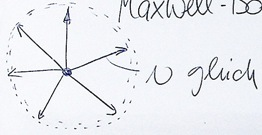
\includegraphics{Bild112} \\
Maxwell-Boltzmann-Geschwindigkeitsverteilung \\
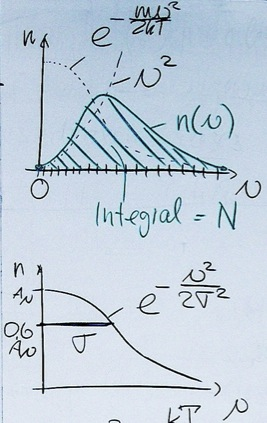
\includegraphics{Bild113}
\[ \implies \sigma^2 = \frac{kT}{m} \]

\subsection{Der Gasdruck}
Model \\
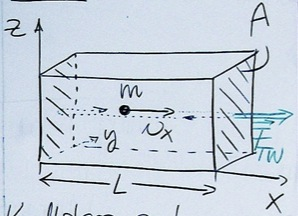
\includegraphics{Bild114} \\
Kraftstoss auf Wand:
\[ \Delta p_x = 2 m v_x = \int F_{TW} \cdot \dd t \]
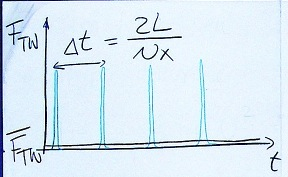
\includegraphics{Bild115}
\[
	\Delta p_x = \overline{F_{TW}} \cdot \Delta t = \overline{F_{TW}} \cdot \frac{2L}{v_x} \\
	\overline{F_{TW}} = \frac{m v_x^2}{L}
\]
$N$ Teilchen \\
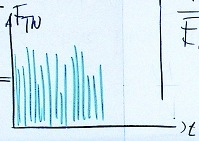
\includegraphics{Bild116} \\
$\implies$ Brownsche Bewegung \\
Druck $p$:
\[
	p = \frac{\overline{F_{TW}}}{A} \cdot N \cdot \underbrace{\frac{1}{3}}_{\text{Bewegung in $x$-Richtung}} \\
	p = \frac{1}{3} N \frac{m \overline{v}^2}{V} \\
	\overline{E_{\text{kin}}} = \frac{1}{2} m \overline{v}^2 \\
	\implies p = \frac{2}{3} \frac{N}{V} \overline{E_{\text{kin}}}
\]

\section{Temperatur}
\dots was ist das eigentlich? \\
All diese Grössen beschreiben einen bestimmten Zustand des Gases. \\
Zustandsänderungen (äussere Einwirkung) \\
$\implies$ Zustandsgleichung (ideales Gas) \\
Für $\SI{1}{\mole} = 6.02 \cdot 10^{23}$ Teilchen $= N_A$ (Avogadro-Konstante)
\[ p \cdot V = R \cdot T \]
$R$: universelle Gaskonstante
\begin{def*}
	\[ \SI{1}{\mole} \ce{^{12} C} \corresponds \SI{12.0}{\gram} \]
\end{def*}
\[ R = \SI{8.31}{\joule\per\mole\kelvin} \]
$T$ in Kelvin!
\begin{bsp*}[ note = {Volumen verringern ($T$ = konst.)} ]
	\[ p = \frac{RT}{V} \]
\end{bsp*}
\begin{bsp*}[ note = {Abkühlen ($p$ = konst.)} ]
	\[ V = \frac{R}{p} \cdot T \]
\end{bsp*}
Für $\nu$ mole:
\[ p \cdot V = \nu \cdot R \cdot T \]
Für Gasgemische:
\[
	\nu_1 , \nu_2 , \nu_3 , \dots \text{ mole} \\
	\implies pV = ( \nu_1 , \nu_2 , \nu_3 + \dots ) \cdot RT
\]
Partialdruck:
\[
	p_i = \nu_i \cdot \frac{RT}{V}
	\intertext{mit}
	p = p_1 + p_2 + p_3 + \dots
\]

\begin{rep*}[ note = Thermodynamik ]
	Modell des idealen Gases \\
	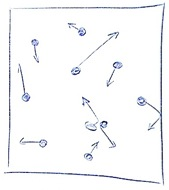
\includegraphics{Bild117} \\
	$N$ Teilchen ($10^{23}$!) \\
	$m_i , \vec{r_i}(t) , \vec{v_i}(t)$
	Zustand des Gases:
	\begin{itemize}
		\item Innere Energie
			\[ U = \sum_{i = 1}^N \frac{1}{2} m_i v_i^2 \]
		\item Mittlere kinetische Energie pro Teilchen:
			\[ \overline{E_{\text{kin}}} = \frac{U}{N} \]
		\item Gasdruck:
			\[ p = \frac{2}{3} \frac{N}{V} \overline{E_{\text{kin}}} \]
		\item Temperatur: \dots
		\item Maxwell-Boltzmann-Geschwindigkeitsverteilung \\
			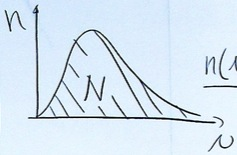
\includegraphics{Bild118}
			\[ n(v) = A_v v^2 e^{-\frac{m v^2}{2kT}} \]
			Stellt sich durch Stösse ein!
	\end{itemize}
	
	Zustandsgleichung
	\[ p \cdot V = \underbrace*{\nu}_{\text{Anzahl Mole}} \cdot \underbrace*{R}_{\text{universelle Gaskonstante } = \SI{8.31}{\joule\per\mole\kelvin}} \cdot T \]
\end{rep*}

\subsection{Was ist Temperatur}
\begin{def*}[ note = thermodynamisches Gleichgewicht , index = thermodynamisches Gleichgewicht , indexformat = {12 2!1~} ]
	Zustandsgrössen sind zeitlich konstant
\end{def*}
\begin{bsp*}[ note = 2 Körper (auch Gase) ]
	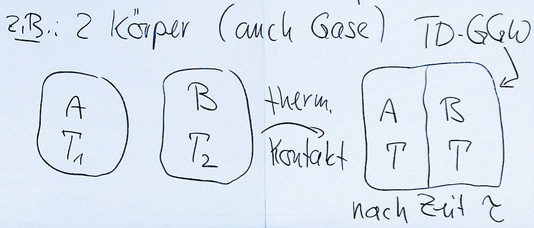
\includegraphics{Bild119}
\end{bsp*}

\subsection{Wärmeaustausch}
\begin{itemize}
	\item Berührung (Wärmeleitung)
	\item Wärmestrahlung ($\rightarrow$ später)
\end{itemize}
$\rightarrow$ Temperaturmessung!

\subsubsection{Temperatur beim idealen Gas}
\[
	\SI{1}{\mole}: \\
	p \cdot V = RT \\
	p \cdot V = \frac{2}{3} N_A \overline{E_{\text{kin}}} \\
	\implies \overline{E_{\text{kin}}} = \frac{3}{2} \frac{R}{N_A} T = \frac{3}{2} \underbrace{k}_{\text{Boltzmann-Konstante} = \SI{1.38E-23}{\joule\per\kelvin}} T \\
	\implies \text{Temperatur $\approx$ Energie} \\
	\implies \overline{E_{\text{kin}}} = \frac{1}{2} \overline{m v^2} = \frac{3}{2} kT
\]

TD-GGW: weitere Situation
\section{Diffusion}
\begin{enumerate}
	\item 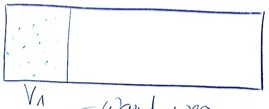
\includegraphics{Bild120} \\
		$N$ Teilchen TD-GGW
	\item 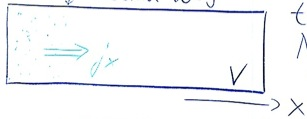
\includegraphics{Bild121} \\
		$t = 0$ \\
		Nicht-GGW, zeitlich veränderlich Diffusionsstromdichte $j_x$
	\item 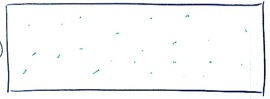
\includegraphics{Bild122} \\
		$t = \tau$ \\
		TD-GGW
\end{enumerate}

\subsection{Quantitative Beschreibung}
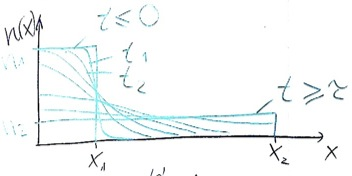
\includegraphics{Bild123} \\
alles gleiche Fläche \\
Teilchendichte $n(x)$ \\
zeitliche Änderung von $n(x)$ \\
Ursache: Dichtegefälle
\begin{enumerate}
	\item \[ n_1 = \frac{N}{V_1} \]
	\item \[ [ j_x ] : \si{Teilchen \per\metre\squared\second} \]
	\item \[ n_2 = \frac{N}{V} \]
\end{enumerate}
\[ j_x = -D \cdot \frac{\dd n}{\dd x} \]
Fick'sche Diffusionsgleichung \\
$D$: Diffusionskonstante
\[ [ D ] = \si{\metre\squared\per\second} \]
Man findet: $D \sim \underbrace*{\overline{l}}_{\text{mittlere freie Weglänge}} \cdot \underbrace*{\overline{v}}_{\text{mittlere Schnelligkeit}}$ \\
In Lösungen
\[
	\left. \begin{matrix*}[l]
		\text{Konzentration} \\
		c_i = \frac{\nu_i}{V_{\text{Lösg.}}}
	\end{matrix*} \right\} \quad j_x = -D \cdot \frac{\dd c_i}{\dd x}
\]

\subsection{Diffusion durch porösen Ton}
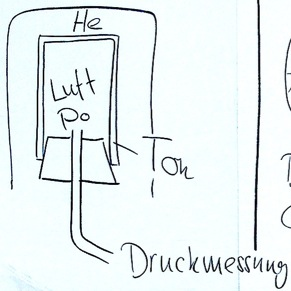
\includegraphics{Bild124} \\

\subsection{Gasaufnahme in Flüssigkeiten}
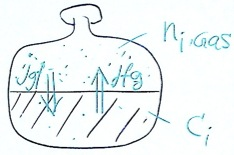
\includegraphics{Bild125} \\
Diffusion Gas $\rightleftarrows$ Flüssigkeitkeit \\
Gleichgewichtskonzentration $c_i^S$ (Sättigungskonzentration)

\subsubsection{Im TD-GGW}
\[ j_{gf} = j_{fg} \]
Prozesse:
$j_{gf}$: 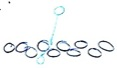
\includegraphics{Bild126} \\
$j_{gf} \sim n_{i,\text{gas}} \sim \underbrace{p_i}_{\text{Partialdruck}}$ \\
$j_{fg}$: 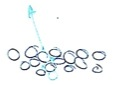
\includegraphics{Bild127} \\
$\implies j_{fg} \sim c_i$ \\
$\implies c_1 \sim p_i$ \\
Henry-Dalton-Gesetz:
\[ c_i^S = K(T) \cdot p_i \]
$K(T)$: Gassorte, Flüssigkeit \\
$K(T) \searrow$ wenn $T \nearrow$

\section{Osmose}
Im TD-GGW \\
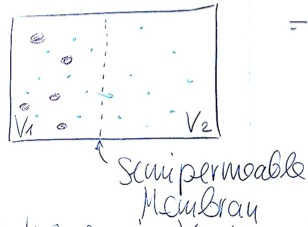
\includegraphics{Bild128} \\
Druck:
\[
	p \cdot V = \nu \cdot R \cdot T \\
	\implies p = \frac{\nu \cdot N_A \cdot k \cdot T}{V} = n \cdot kT \\
	\begin{split}
		\text{Druck }
			&\text{in } V_1 : p = n_\cdot \cdot kT + n_\bullet \cdot kT \\
			&\text{in } V_2 : p = n_\cdot \cdot kT
	\end{split} \\
	\implies \Delta p = n_\bullet kT \quad \text{osmotischer Druck (auch in Lösungen!)}
\]

\begin{rep*}[ note = Diffusion ]
	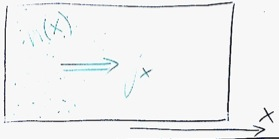
\includegraphics{Bild129}
	\[
		\begin{split}
			\text{Gase: } &j_x = -D \frac{\dd n}{\dd x} \\
			\text{Lösungen: } &j_x = -D \frac{\dd c}{\dd x}
		\end{split}
		\text{Konzentration } c_i = \frac{\nu_i}{V_{\text{Lösg}}}
	\]
	
	Diffusionskonstante
	\[ D \sim \underbrace*{\overline{l}}_{\substack{\text{hohe Dichte}\\\rightarrow \text{ langsam}}} \cdot \underbrace*{\overline{v}}_{\substack{\text{kleine Massen}\\\rightarrow \text{ Schnell}}} \]
	
	Gasaufnahme in Flüssigkeiten \\
	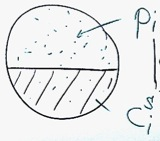
\includegraphics{Bild130}
	\[ c_i^S = K(T) \cdot p_i \]
	
	Osmose \\
	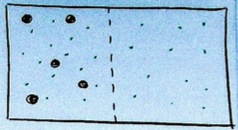
\includegraphics{Bild131}
	\[
		\begin{split}
			\text{Gase: } &\Delta p = n_\bullet \cdot kT \\
			\text{Lösungen: } &p_{\text{osm.}} = c_\bullet \cdot RT
		\end{split} \\
		\left( \text{aus } c_\bullet \cdot R = \frac{\nu}{V} R = \underbrace{\frac{\nu \cdot N_A}{V}}_{n_\bullet} k \right)
	\]
\end{rep*}

\section{Physiologische Kochsalzlösung}
\[
	c_{\text{physio}} = \SI{9}{\gram\per\litre} = \frac{\nu}{V_{\text{Lösg}}} \\
	\text{Molmasse: } m_{\ce{NaCl}} = \SI{23}{\gram} + \SI{35.5}{\gram} = \SI{58.5}{\gram} \corresponds 6.02 \cdot 10^{23} \ce{NaCl} \text{ Paare!} \\
	c = \frac{\SI{9}{\gram\per\litre}}{\SI{58.5}{\gram\per\mole}} \cdot 2 = \SI{0.308}{\mole\per\litre} = \SI{308}{\mole\per\metre\cubed} \\
	p_{\text{osm.}} = c \cdot R \cdot T = \SI{308}{\mole\per\metre\cubed} \cdot \SI{8.31}{\joule\per\mole\kelvin} \cdot \SI{310}{\kelvin} = \SI{7.93E5}{\pascal} \approx \SI{8}{\bar}
\]
Infusion mit reinem Wasser: Hämolyse \\
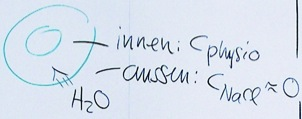
\includegraphics{Bild132}

\section{Der Dampfdruck}
ideales Gas $p = \frac{R \cdot T}{V}$ \\
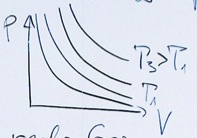
\includegraphics{Bild133} \\
reales Gas \\
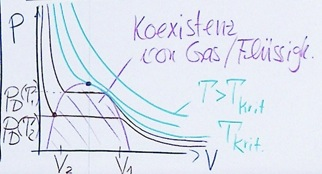
\includegraphics{Bild134} \\
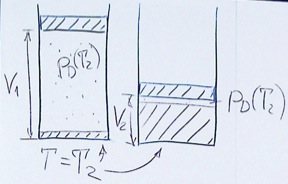
\includegraphics{Bild135} \\
Dampfdruck-Kurve \\
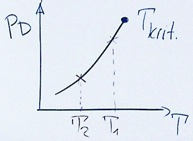
\includegraphics{Bild136} \\
2 Situationen \\
Geschlossenes Gefäss (Kochtopf) \\
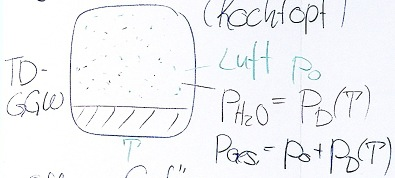
\includegraphics{Bild137} \\
Offenes Gefässe \\
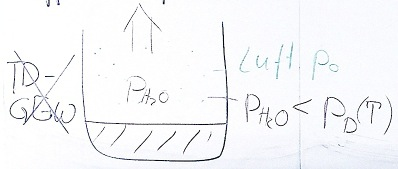
\includegraphics{Bild138}

\section{Luftfeuchtigkeit}
absolute LF $f_a = \frac{m_{\ce{H2O}}}{V}$ in \si{\kilo\gram\per\metre\cubed} \\
relative LF $f_r = \frac{p_{\ce{H2O}}}{p_D(T)}$ in \% \\
$f_r = 100\% \implies$ Kondensation
\[ p_{\ce{H2O}} = \underbrace{\frac{m_{\ce{H2O}}}{M_{\ce{H2O}}}}_{\nu_{\ce{H2O}}} \cdot \frac{R \cdot T}{V} = f_a \cdot \frac{RT}{M_{\ce{H2O}}} \]

\section{1. Hauptsatz der Wärmelehre}
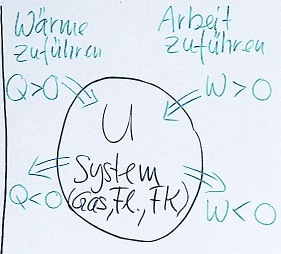
\includegraphics{Bild139} \\
Prozess: Man tut etwas mit dem System
\[ \Delta U = U_{\text{nach Prozess}} - U_{\text{vor Prozess}} = Q + W \]
Wie? z.B. Arbeit \\
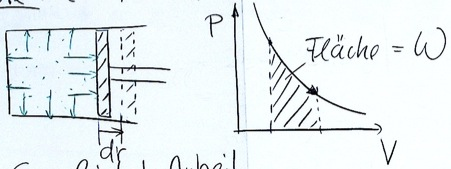
\includegraphics{Bild140} \\
Gas leistet Arbeit $\implies W < 0$

\section{Wärmeleitung}
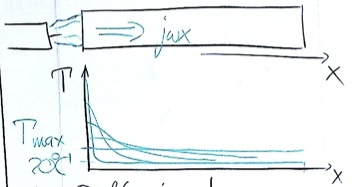
\includegraphics{Bild141} \\
Wie Diffusion!
\[ j_{wx} = -\lambda \cdot \frac{\dd T}{\dd x} \]
$\lambda$ Wärmeleitzahl [ \si{\watt\per\kelvin\metre} ] stark materialabhängig

\begin{bsp*}
	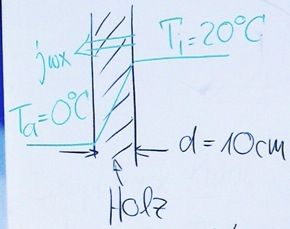
\includegraphics{Bild142}
	\[
		\lambda = \SI{0.1}{\watt\per\kelvin\metre} \\
		j_{wx} = \SI{-0.1}{\watt\per\kelvin\metre} \cdot \frac{\SI{20}{\kelvin}}{\SI{0.1}{\metre}} = \SI{20}{\watt\per\metre\squared}
	\]
\end{bsp*}
\begin{bsp*}[ note = \ce{H2O} ]
	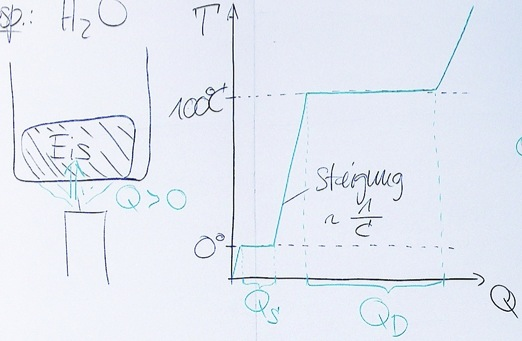
\includegraphics{Bild143} \\
	$Q_S$: Schmelzwärme \SI{6.03}{\kilo\joule\per\mole} \\
	$Q_D$: Verdampfungswärme \SI{40.7}{\kilo\joule\per\mole}
	$\overset{Q > 0}{\implies} T_1 \overset{\tau}{\rightarrow} T_2$ \\
	$\Delta T = \frac{Q}{C}$ Wärmekapazität (des Systems) \\
	molare Wärekapazität $C_{\si{\mole}} = \frac{C}{\nu}$ [ \si{\joule\per\mole\kelvin} ] \\
	$Q$(Wasser von $\SI{0}{\celsius} \rightarrow \SI{100}{\celsius}$) $\approx \SI{8}{\kilo\joule\per\mole}$
\end{bsp*}

\begin{rep*}[ note = 1. Hauptsatz der Wärmelehre ]
	\[ \boxed{\Delta U = Q + W} \quad ( = Q^{\swarrow} + W^{\swarrow} ) \]
\end{rep*}

\begin{bsp*}[ note = \ce{H2O} ]
	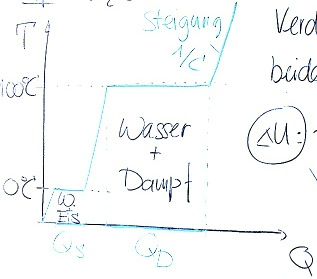
\includegraphics{Bild144} \\
	Schmelzwärme $Q_S$ \\
	Verdampfungswärme $Q_D$ \\
	beides Umwandlungswärmen \\
	$\Delta U$:
	\begin{itemize}[ label = $\rightarrow$ ]
		\item Temeraturzunahme $\Delta T = \frac{Q}{C}$ ( $E_{\text{kin}} = \frac{3}{2} kT$ )
		\item Phasenumwandlung ( umgekehrt beim Ankühlen )
	\end{itemize}
	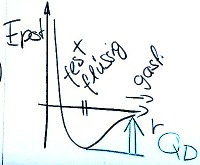
\includegraphics{Bild145}
\end{bsp*}

\section{2. Haupsatz der WL}
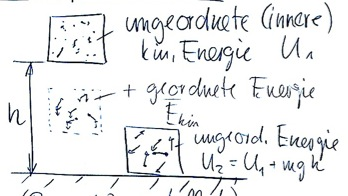
\includegraphics{Bild146} \\
\begin{bsp*}
	Wasserfall
\end{bsp*}
\textbf{Prozess ist irreversibel!}

2. HS: Welcher Anteil an ungeordneter Energie lässt sich wieder in geordnete Energie umwandeln?
\begin{def*}[ note = Entropie , index = Entropie S , indexformat = {1 2} ]
	\textbf{Entropie $S$} = Mass \textbf{für die Unordnung}
\end{def*}
Antwort: freie Energie $\boxed{F = U - TS}$
